\documentclass{TIJMUjiaoanLL}
\pagestyle{empty}


\begin{document}


%课程名称
\kecheng{Linux系统概论}
%课程内容
\neirong{Linux基础\ /\ 第1\&2章}
%教师姓名
\jiaoshi{伊现富}
%职称
\zhicheng{讲师}
%教学日期(格式:XXXX年XX月XX日XX时-XX时)
\riqi{2018年5月7日10:00-12:00}
%授课对象(格式:XXX系XXXX年级XX班(硕/本/专科))
\duixiang{生物医学工程与技术学院2016级生信班(本)}
%听课人数
\renshu{28}
%授课方式
\fangshi{理论讲授}
%学时数
\xueshi{2}
%教材版本
\jiaocai{Unix入门经典,第1版}


%教案首页
\firstHeader
\maketitle
\thispagestyle{empty}

\mudi{
\begin{itemize}
  \item 掌握Linux的两层含义;Linux操作系统的组件;登录、退出Linux的基本方法;查看联机帮助页的方法。
  \item 熟悉常见的Linux发行版。
  \item 了解Linux的发展简史;Linux的应用领域。
  \item 自学Linux的安装;Linux的网络资源。
\end{itemize}
}

\fenpei{
\begin{itemize}
  \item (5')引言与导入:提问熟悉的常见操作系统,比较Windows、Linux和Mac三大操作系统。
  \item (45')Linux简介:回顾Linux的发展简史,讲解Linux的两层含义,总结Linux系统的优缺点,介绍常见的Linux发行版,展示Linux的应用领域。
  \item (15')操作系统组件:分析Linux系统的构成组件及各个组件的功能,介绍常见的shell。
  \item (15')Linux的学习:介绍Linux系统的安装方法,比较图形用户界面(GUI)和命令行界面(CLI),总结学习Linux的策略、步骤和方法。
  \item (15')Linux起步:介绍不同环境下登录Linux的方法,讲解登录和退出Linux的各种命令,讲解查看联机帮助页的man命令及其结果的解读。
  \item (5')总结与答疑:总结授课内容中的知识点与技能,解答学生疑问。
\end{itemize}
}

\zhongdian{
\begin{itemize}
  \item 重点:远程登录Linux的方法,查看联机帮助页的方法。
  \item 难点:Linux的两层含义。
  \item 解决策略:通过讲解历史背景和实例演示帮助学生理解、记忆。
\end{itemize}
}

\waiyu{
  \vspace*{-10pt}
  \begin{multicols}{2}
    Linux内核(Linux Kernel)

    GNU通用公共许可协议(GPL)

    Linux发行版(Linux distribution)

    图形用户界面(Graphical User Interface,GUI)

    命令行界面(Command Line Interface,CLI)

    联机帮助页(man pages)
  \end{multicols}
  \vspace*{-10pt}
}

\fuzhu{
\begin{itemize}
  \item 多媒体:Windows、Linux和Mac三大系统的比较,Linux的发展简史,Linux的标准发音,常见的Linux发行版,Linux的应用领域,Linux系统的构成组件,GUI和CLI的比较。
  \item 板书:Linux的两层含义,常见的shell种类。
  \item 演示:登录、退出Linux以及查看联机帮助页的命令。
\end{itemize}
}

\sikao{
  \vspace*{-10pt}
  \begin{multicols}{2}
  \begin{itemize}
    \item Unix和Linux分别是由谁开发的?
    \item Linux发行版主要分成哪两大系统?
    \item 列举几个常见的Linux发行版。
    \item Linux操作系统主要包括哪些组件?
    \item 列举几种常见的shell。
    \item 登录、退出、关闭Linux的常用命令。
    \item 如何查看命令的联机帮助页?
    \item 如何根据关键字查找相关命令?
  \end{itemize}
  \end{multicols}
  \vspace*{-10pt}
}

\cankao{
\begin{itemize}
  %\item (美)Paul Love,Joe Merlino\ 等著,张楚雄,许文昭\ 译。Unix入门经典,清华大学出版社,2006。
  \item (美)Harley Hahn\ 著,张杰良\ 译。Unix \& Linux大学教程,清华大学出版社,2010。
  \item 鸟哥\ 著,王世江\ 改编。鸟哥的Linux私房菜——基础学习篇(第三版),人民邮电出版社,2010。
  \item 维基百科等网络资源。
\end{itemize}
}

\firstTail


%教案续页
\newpage
\otherHeader

\begin{enumerate}
  \item 引言与导入(5分钟)
    \begin{enumerate}
      \item 三大操作系统
	\begin{itemize}
\parpic[fr]{
\includegraphics[width=6cm]{c1.os.15.jpg}}
	  \item Windows:was designed to please accountants
	  \item Unix/Linux:was designed to please programmers
	  \item Mac:was designed to please users
	\end{itemize}
    \end{enumerate}

  \item Linux简介(45分钟)
    \begin{enumerate}
      \item Linux发展简史
	\begin{itemize}
          \item 1969,Ken Thompson(肯\textbullet 汤普逊),Unics $\Rightarrow$ Unix
          \item 1973,Ken Thompson \& Dennis Ritchie(丹尼斯\textbullet 里奇),用C语言重写Unix
          \item 1977,Bill Joy(比尔\textbullet 乔依),BSD(Berkeley Software Distribution)
	  \item 1985,Richard Stallman(理查德\textbullet 斯托曼),GNU(GNU's Not Unix)
          \item 1987,Andrew Tanenbaum(安德鲁\textbullet 谭宁邦),Minix
          \item 1989,Richard Stallman,GPL(GNU General Public License)
          \item 1991,Linux Torvalds(林纳斯\textbullet 托瓦兹),Linux
          \item 1995,Red Hat(红帽公司)成立
          \item 1996,Larry Ewing(拉里\textbullet 厄文),Linux吉祥物——Tux
          \item 2004,Canonical公司成立
          \item 2007,Google发布Android的源代码
          \item 2008,第一部Android智能手机发布
	\end{itemize}
      \item Linux操作系统
	\begin{enumerate}
	  \item \textcolor{red}{\textbf{【难点】}}Linux的两层含义\textcolor{red}{(结合Linux的发展历史进行讲解)}
	    \begin{itemize}
	      \item Linux内核:包括内核及内核工具,GPL授权,兼用于Unix
	      \item Linux系统:基于Linux内核的类Unix系统,Linux内核+shell+实用工具
	    \end{itemize}
	  \item Linux的特色和优缺点
	    \begin{itemize}
	      \item 特色:自由开放,配置低廉,强大稳定,独立作业
	      \item 优点:稳定性,安全性,免费,多任务、多用户,可移植性,灵活性,……
	      \item 缺点:厂商支持,游戏支持,专业软件,……
	    \end{itemize}
	\end{enumerate}
\item Linux发行版\textcolor{red}{(与品牌电脑/手机相类比)}
	\begin{enumerate}
	  \item Linux发行版 = Linux内核 + 实用工具 + 编程工具 + GUI
	  \item Linux发行版的两大系统
	    \begin{itemize}
	      \item Red Hat系:RHEL,CentOS,Fedora,SUSE/openSUSE,……
	      \item Debian系:Debian,Ubuntu,Linux Mint,Deepin,……
	    \end{itemize}
	  \item Linux发行版的选择
	    \begin{itemize}
\parpic[fr]{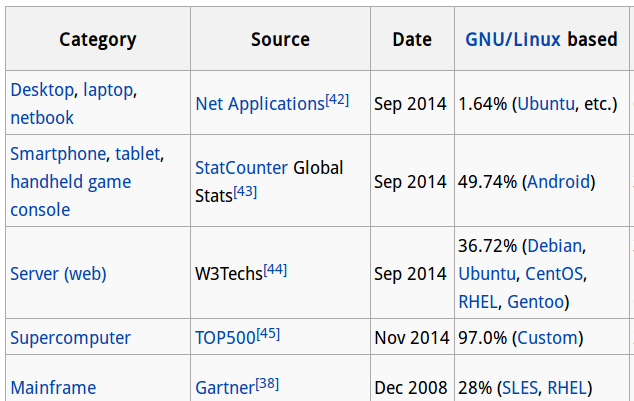
\includegraphics[width=9cm]{c1.linux.area.all.png}}
	      \item 企业环境:RHEL,SUSE,……
	      \item 服务器环境:CentOS,openSUSE,……
	      \item 桌面环境:Ubuntu,Fedora,Linux Mint,Deepin,Gentoo,……
	    \end{itemize}
	\end{enumerate}
      \item Linux的应用领域:广泛
	\begin{itemize}
	  \item 桌面环境:微乎其微
	  \item 服务器:三分之二
	  \item 智能手机:半壁江山
	  \item 超级计算机:独领风骚
	\end{itemize}
    \end{enumerate}

\otherTail
\newpage
\otherHeader

  \item 操作系统组件(15分钟)
    \begin{enumerate}
\parpic[fr]{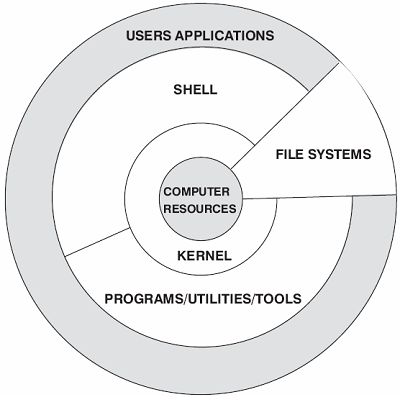
\includegraphics[width=5.5cm]{c1.system.parts.01.png}}
      \item 系统组件:内核 + shell + 文件系统 + 实用程序
      \item 内核
	\begin{itemize}
	  \item 概述:操作系统的核心,控制计算机
	  \item 功能:内存管理,进程管理,输入输出,文件管理,……
	  \item 版本:3.A.B,A为内核版本,B为安全补丁
	\end{itemize}
      \item shell
	\begin{itemize}
	  \item 概述:命令行解释器,使用户与操作系统进行交互
	  \item 种类:sh,bash,dash,ksh,zsh,csh,……
	\end{itemize}
      \item 文件系统:组织文件和目录
      \item 实用程序:各种应用程序
    \end{enumerate}

  \item Linux的学习(15分钟)
    \begin{enumerate}
      \item Linux的安装:Live CD,Live USB,硬盘安装(虚拟机,多重引导系统,单系统)
      \item Linux的学习
	\begin{itemize}
\parpic[fr]{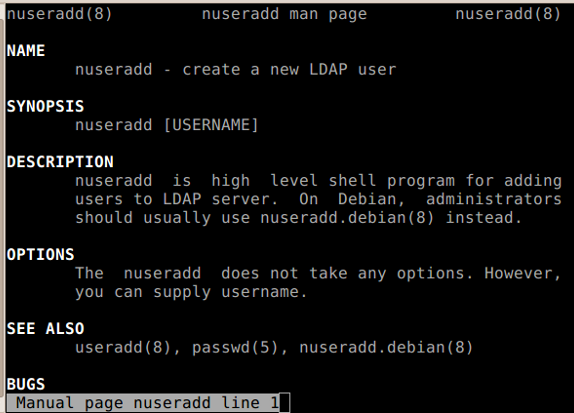
\includegraphics[width=7cm]{c1.man.page.02.png}}
	  \item GUI vs. CLI
	  \item 策略:学习 + 摸索 + 实践 + 总结
	  \item 内容:安装与命令,用户和组,权限管理,Vim编辑器,shell脚本,软件管理,……
	  \item 方法:忘记Windows,CLI是本质,自力更生,先尝试、再查询、后提问
	\end{itemize}
    \end{enumerate}

  \item
    \textcolor{red}{\textbf{【重点】}}Linux起步(15分钟)\textcolor{red}{(通过实例进行演示)}
    \begin{enumerate}
      \item 登录Linux:\textcolor{red}{ssh},telnet,\textcolor{red}{sftp},ftp
      \item 退出Linux:logout,shutdown,reboot
      \item 联机帮助页:\textcolor{red}{man},man -k
    \end{enumerate}

      %\begin{figure}[h]
        %\centering
        %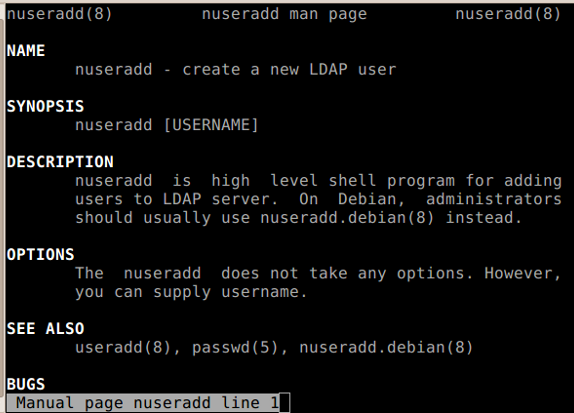
\includegraphics[width=7cm]{c1.man.page.02.png}
        %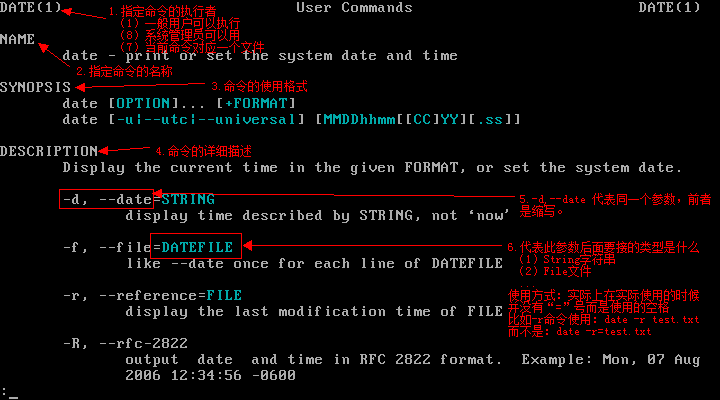
\includegraphics[width=9cm]{c1.man.page.01.png}
      %\end{figure}

  \item 总结与答疑(5分钟)
    \begin{enumerate}
\parpic[fr]{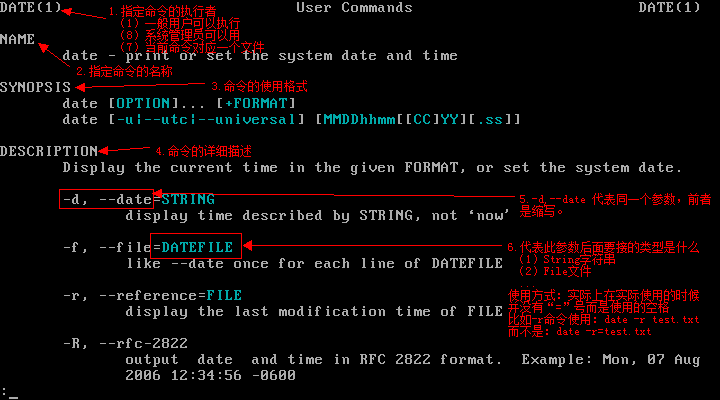
\includegraphics[width=11.3cm]{c1.man.page.01.png}}
      \item 知识点
	\begin{itemize}
	  \item Linux的历史与现状
	  \item Linux的两层含义
	  \item 常见的Linux发行版
	  \item Linux系统组件
	  \item Linux的登录与退出
	  \item 查看联机帮助页
	\end{itemize}
      \item 技能
	\begin{itemize}
	  \item VirtualBox的使用
	  \item Linux的安装
	  \item 由浅入深学习Linux
	\end{itemize}
    \end{enumerate}
\end{enumerate}

\otherTail


\end{document}

